\chapter{A Two-dimensional Transient Conduction Problem}
The four materials problem is a two-dimensional transient conduction problem. It consists in a long rod composed of four different materials with different properties. The general scheme of the problem is represented in figure \ref{fourmaterials}, and the dimensions of the materials, their properties, and the boundary conditions are in the tables below.
\begin{figure}[h]
	\centering
	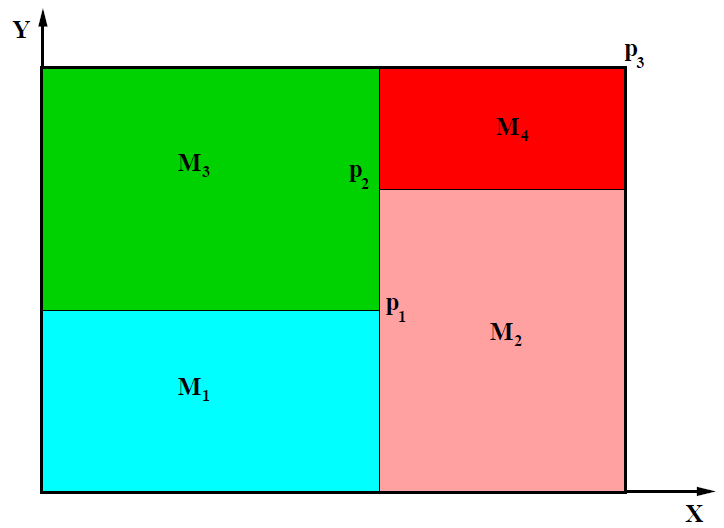
\includegraphics[scale = 0.6]{FourMaterials/Fourmaterials}
	\caption{General scheme of the four materials problem}
	\label{fourmaterials}
\end{figure}
\begin{table}[h!]
	\centering
	\begin{tabular}{ |c|c|c|}
		\hline
		  & x [m] & y [m] \\ \hline
		 $p_{1}$ & $0.50$ & $0.40$ \\ \hline
		 $p_{2}$ & $0.50$ & $0.70$ \\ \hline
		 $p_{3}$ & $1.10$ & $0.80$ \\ \hline
	\end{tabular}
\caption{Problem coordinates}
\end{table}
\begin{table}[h!]
	\centering
	\begin{tabular}{ |c|c|c|c| }
		\hline
		& $\rho [kg/m^{3}]$ & $c_{P} [J/kgK]$ & $\lambda [W/mK]$ \\ \hline
		$M_{1}$ & $1500.00$ & $750.00$ & $170.00$ \\ \hline
		$M_{2}$ & $1600.00$ & $770.00$ & $140.00$ \\ \hline
		$M_{3}$ & $1900.00$ & $810.00$ & $200.00$ \\ \hline
		$M_{4}$ & $2500.00$ & $930.00$ & $140.00$ \\ \hline
	\end{tabular}
\caption{Physical properties of the materials}
\end{table}
\begin{table}
	\centering
	\begin{tabular}{ |c|c|}
		\hline
		Cavity wall & Boundary condition \\ \hline
		Bottom & Isotherm at $T=23.00 ^{\circ}C$ \\ \hline
		Top & Uniform $Q_{flow}=60.00 W/m$ length \\ \hline
		Left & In contact with a fluid at $T_{g}=33.00 ^{\circ}C$ and heat transfer coefficient $9.00 W/m^{2}K$ \\ \hline
		Right & Uniform temperature $T=8.00+0.005t ^{\circ}C$ (where $t$ is the time in seconds) \\ \hline
	\end{tabular}
\caption{Boundary conditions}
\end{table}

The initial temperature field is $T=8.00 ^{\circ}C$.

\section{Discretization}
The spatial discretization of the problem is that described in section \ref{SpatialDiscretizationConduction}, and the temporal discretization the one described in section \ref{TemporalDiscretizationConduction}.

\section{Boundary conditions}
The coefficients of the discretized equation in the inner nodes are the ones of the section \ref{DiscrCond}. The outer walls of the rod have special conditions, so each of them has to be studied in order to determine which coefficients of their boundary nodes are different.

In the left wall, there is convection with the fluid outside of the road. In order to fulfil this condition, some coefficients have to be recalculated:
\begin{equation}
a_{W}=0
\end{equation}
\begin{equation}
a_{P}=a_{E}+a_{W}+a_{N}+a_{S}+\frac{\rho_{P}V_{P}\bar{c}_{P}}{\Delta t}+\frac{\beta}{\frac{1}{\alpha}+\frac{d_{Pw}}{\lambda_{P}}}
\end{equation}
\begin{multline}
b_{P}=\frac{\rho_{P}V_{P}\bar{c}_{P}T_{P}^{n}}{\Delta t}+\beta\left(\dot{q}_{vP}^{n+1}V_{P}+\frac{T_{g}}{\frac{1}{\alpha}+\frac{d_{Pw}}{\lambda_{P}}}\right) \\
+\left(1-\beta\right)\left[\frac{T_{g}-T_{P}}{\frac{1}{\alpha}+\frac{d_{Pw}}{\lambda_{P}}}+\lambda_{e}\frac{T_{E}-T_{P}}{d_{PE}}S_{e}-\lambda_{s}\frac{T_{P}-T_{S}}{d_{PS}}S_{s}+\lambda_{n}\frac{T_{N}-T_{P}}{d_{PN}}S_{n}+\dot{q}_{vP}V_{P}\right]^{n}
\end{multline}

There is a constant heat flux in the top wall. The value of this flux is given for the total wall, so it is assumed that it is uniformly distributed over the top wall. In this case, the coefficients that change their value are:
\begin{equation}
a_{N}=0
\end{equation}
\begin{multline}
b_{P}=\frac{\rho_{P}V_{P}\bar{c}_{P}T_{P}^{n}}{\Delta t}+\beta\dot{q}_{vP}^{n+1}V_{P}+Q_{flow}\frac{S_{n}}{S_{top}} \\
+\left(1-\beta\right)\left[-\lambda_{w}\frac{T_{P}-T_{W}}{d_{PW}}S_{w}+\lambda_{e}\frac{T_{E}-T_{P}}{d_{PE}}S_{e}-\lambda_{s}\frac{T_{P}-T_{S}}{d_{PS}}S_{s}+\dot{q}_{vP}V_{P}\right]^{n}
\end{multline}

In the right wall, the temperature $T_{r}$ is given, and it changes over time. The coefficients are very similar to those of the general case. The only differences are:
\begin{equation}
a_{E}=0
\end{equation}
\begin{equation}
a_P=a_{E}+a_{W}+a_{N}+a_{S}+\frac{\rho_{P}V_{P}\bar{c}_{P}}{\Delta t}+\beta\frac{\lambda_{P}S_{e}}{d_{Pe}}
\end{equation}
\begin{multline}
b_{P}=\frac{\rho_{P}V_{P}\bar{c}_{P}T_{P}^{n}}{\Delta t}+\beta\left(\dot{q}_{vP}^{n+1}V_{P}+\frac{\lambda_{P}S_{e}}{d_{Pe}}T_{r}^{n+1}\right) \\
+\left(1-\beta\right)\left[-\lambda_{w}\frac{T_{P}-T_{W}}{d_{PW}}S_{w}+\lambda_{P}\frac{T_{r}-T_{P}}{d_{Pe}}S_{e}-\lambda_{s}\frac{T_{P}-T_{S}}{d_{PS}}S_{s}+\lambda_{n}\frac{T_{N}-T_{P}}{d_{PN}}S_{n}+\dot{q}_{vP}V_{P}\right]^{n}
\end{multline}

Finally, in the bottom wall, the temperature $T_{b}$ is also given, but it is constant over time. The approach is very similar to that of the right wall, so that the different coefficients are:
\begin{equation}
a_{S}=0
\end{equation}
\begin{equation}
a_P=a_{E}+a_{W}+a_{N}+a_{S}+\frac{\rho_{P}V_{P}\bar{c}_{P}}{\Delta t}+\beta\frac{\lambda_{P}S_{s}}{d_{Ps}}
\end{equation}
\begin{multline}
b_{P}=\frac{\rho_{P}V_{P}\bar{c}_{P}T_{P}^{n}}{\Delta t}+\beta\left(\dot{q}_{vP}^{n+1}V_{P}+\frac{\lambda_{P}S_{s}}{d_{Ps}}T_{b}\right) \\
+\left(1-\beta\right)\left[-\lambda_{w}\frac{T_{P}-T_{W}}{d_{PW}}S_{w}+\lambda_{e}\frac{T_{E}-T_{P}}{d_{PE}}S_{e}-\lambda_{P}\frac{T_{P}-T_{b}}{d_{Ps}}S_{s}+\lambda_{n}\frac{T_{N}-T_{P}}{d_{PN}}S_{n}+\dot{q}_{vP}V_{P}\right]^{n}
\end{multline}

\section{Algorithm}
The algorithm used in this convection problem is represented below. In this case, some of the discretization coefficients are constant, but sometimes they are not. These would change slightly the algorithm used.
\begin{figure}
	\centering
	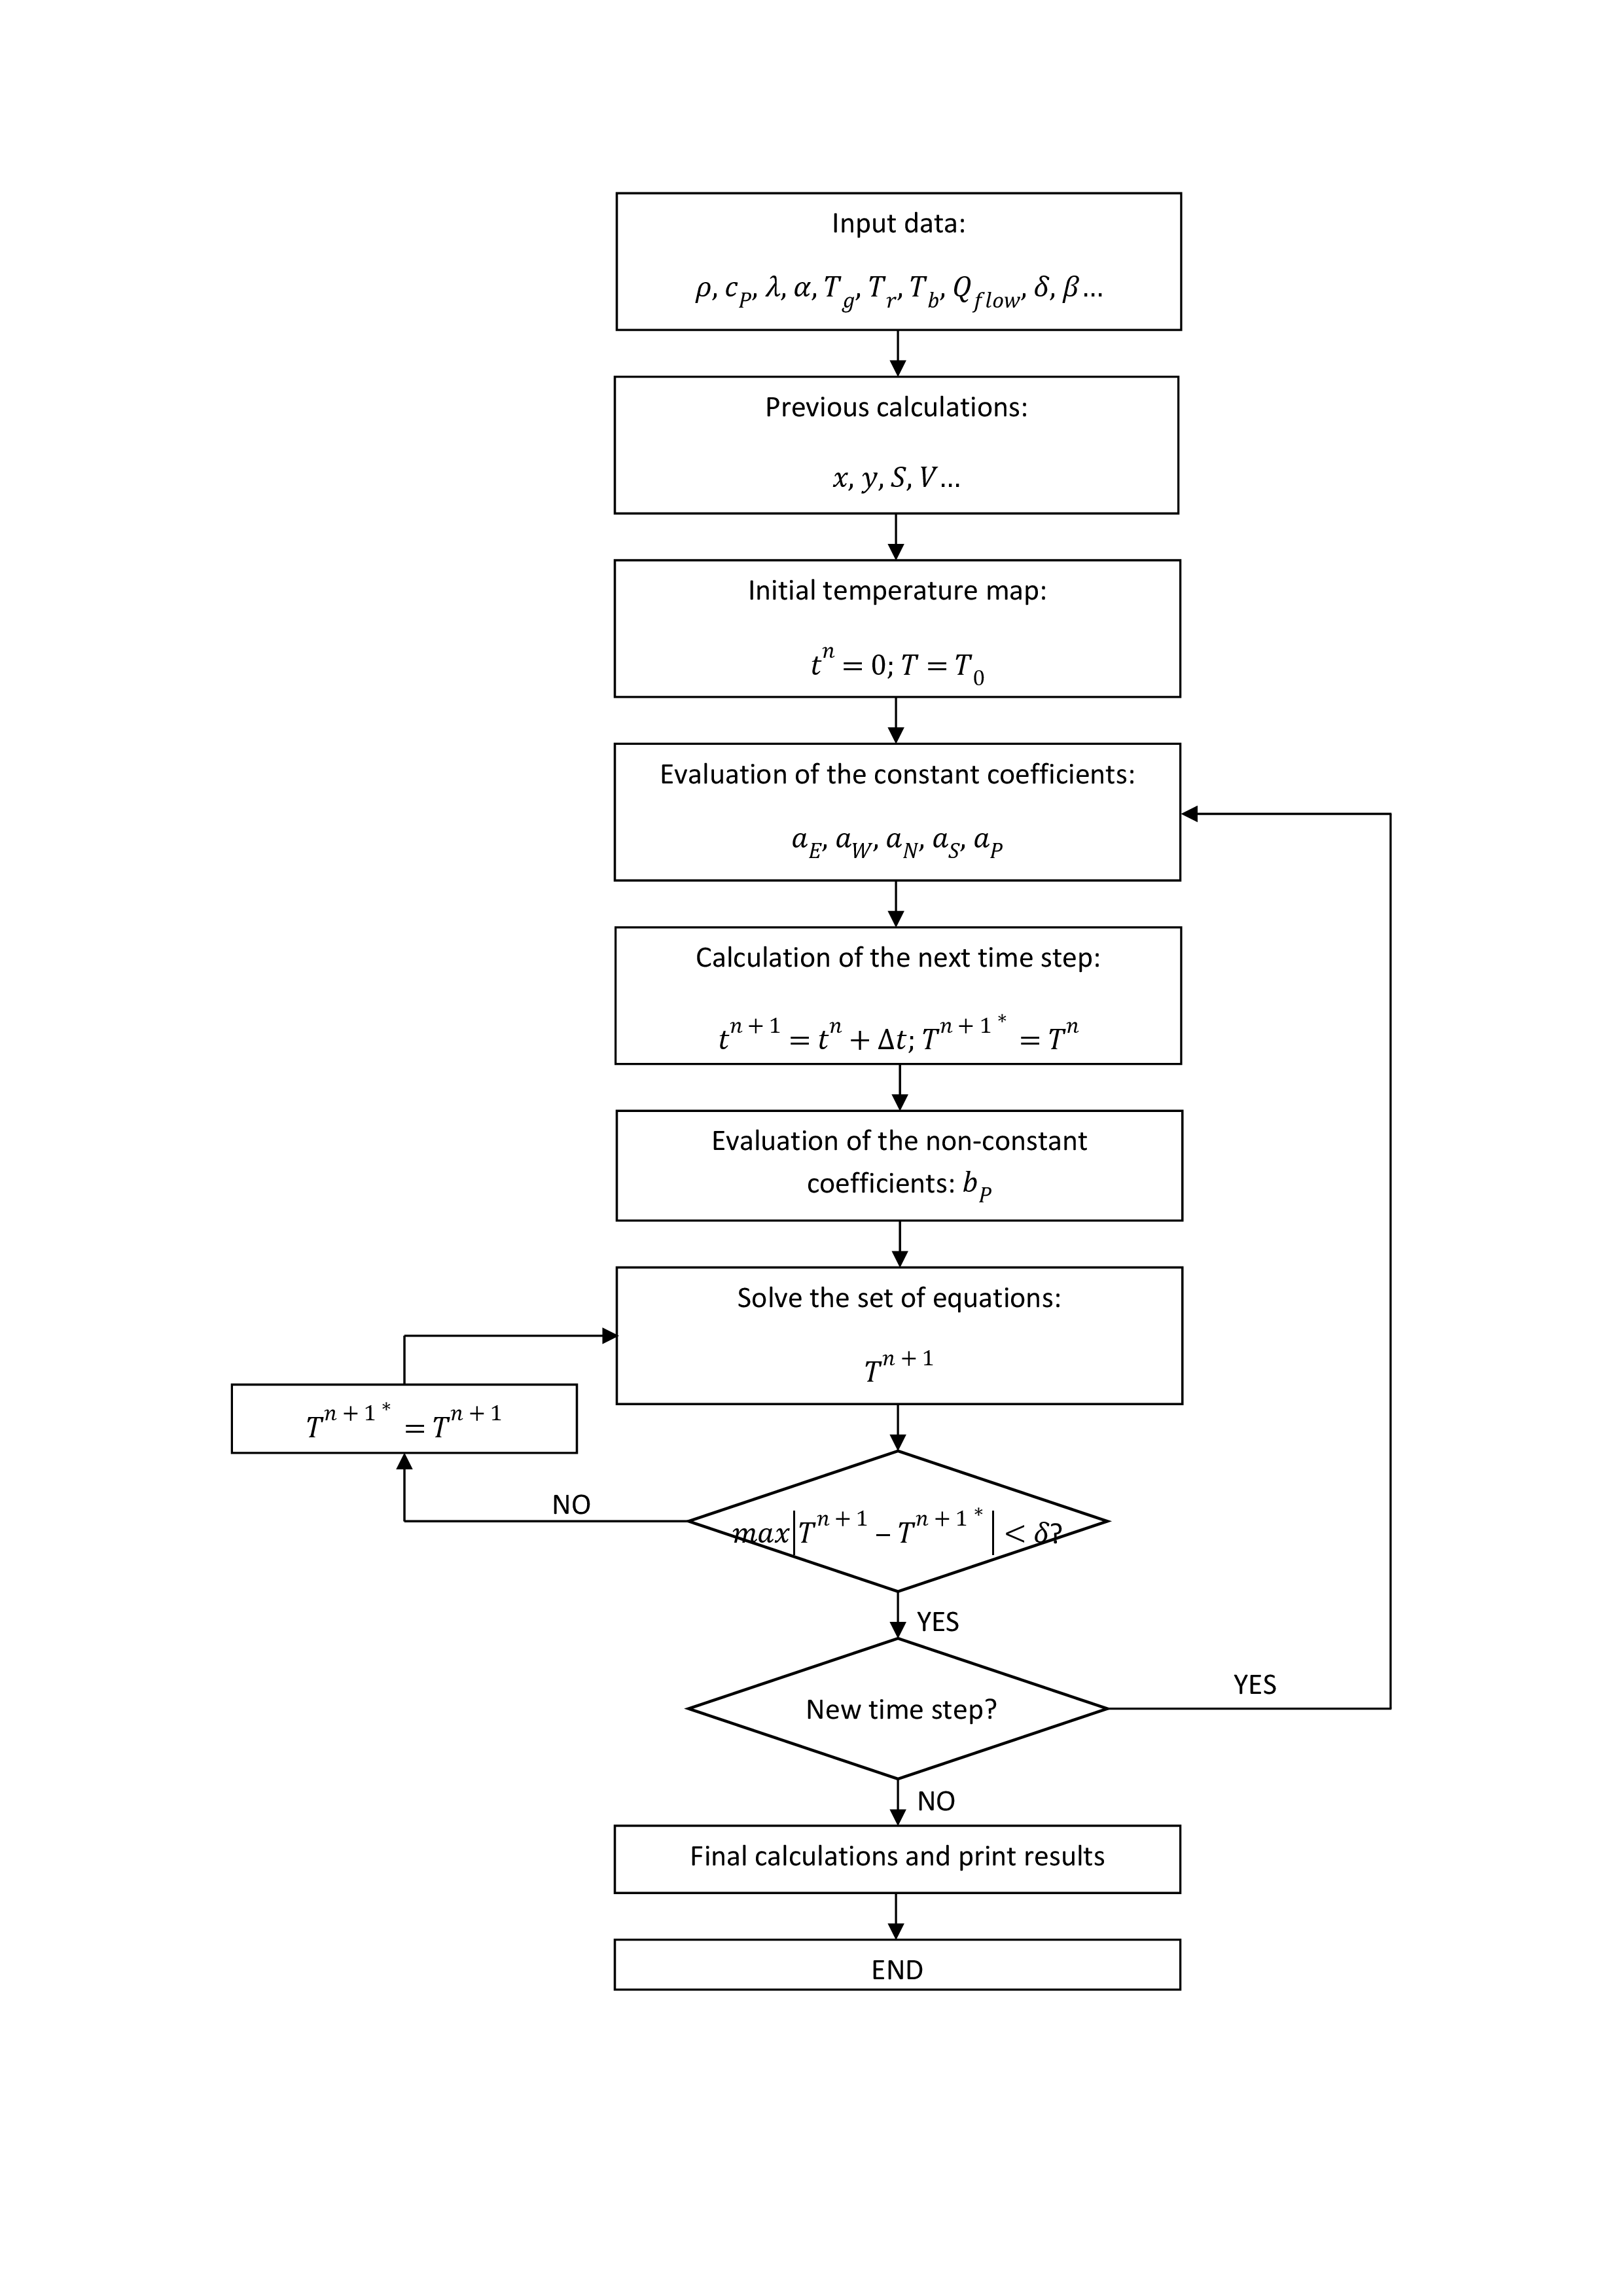
\includegraphics[scale=0.21]{FourMaterials/algorithm}
\end{figure}

\section{Results}